\documentclass[10pt,twocolumn,a4j]{jarticle}
\usepackage{bm}
\usepackage{siunitx}
\usepackage{cases}
\usepackage[japanese]{babel}
\usepackage[dvipdfmx]{graphicx}
\usepackage{subfig}
\columnsep 3zw
\usepackage[dvipdfmx]{graphicx}
\usepackage{subfig} 
\title{A~Computational~Model~of~Cell~Migration~of~Fish~Keratocytes}
\author{生体情報システム研究~~徳永~優}
\date{}
\begin{document}
\maketitle
\section{はじめに}
魚類表皮細胞ケラトサイトは通常時には円形状であるが、細胞遊走時には半月状の形態に変形し(図\ref{fig:kera})、その形態を維持した状態で移動する。この現象は、細胞の変形がケラトサイトの細胞遊走を実現するために重要な特徴であることを示唆している。しかし、半月状形態がどのようなメカニズムにより形成され、維持されるのかは明らかになっていない。本研究の目的は、ケラトサイトが半月状形態を形成、維持する細胞内メカニズムを物理シミュレーション実験により解明することである。
\section{ケラトサイトの細胞遊走}
ケラトサイトが細胞遊走を行う際、細胞骨格であるアクチン分子が重合してFilamentous actin~(F-actin)を形成することによって細胞膜の方向へ伸長することが報告されており、これが細胞膜の変形および細胞の推進のための原動力になることが示唆されてきた\cite{svitkina1997analysis}。アクチン分子の重合には極性があり、F-actinの一定の端でしか起こらない。アクチン分子は、細胞の前方に多く存在し、また、アクチン分子濃度が高い場所であるほど重合の効率が良い\cite{yumura1998spatiotemporal}。重合が起こらない端では逆に、F-actinからアクチン分子が解離していく脱重合が起こっている。細胞後部には左右に広がるストレスファイバー(SF)が細胞遊走時に形成され、細胞内のアクチン分子を引き戻すアクチンレトログレードフロー(ARF)も報告されている\cite{nakashima2015molecular}。ARFに関して、SFの方向へアクチン分子を引き戻すとともに、アクチン分子の重合方向を調整する配向効果も報告されている\cite{swaminathan2017actin}。
\section{シミュレーション手法}
\begin{figure}[tbp]
\centering
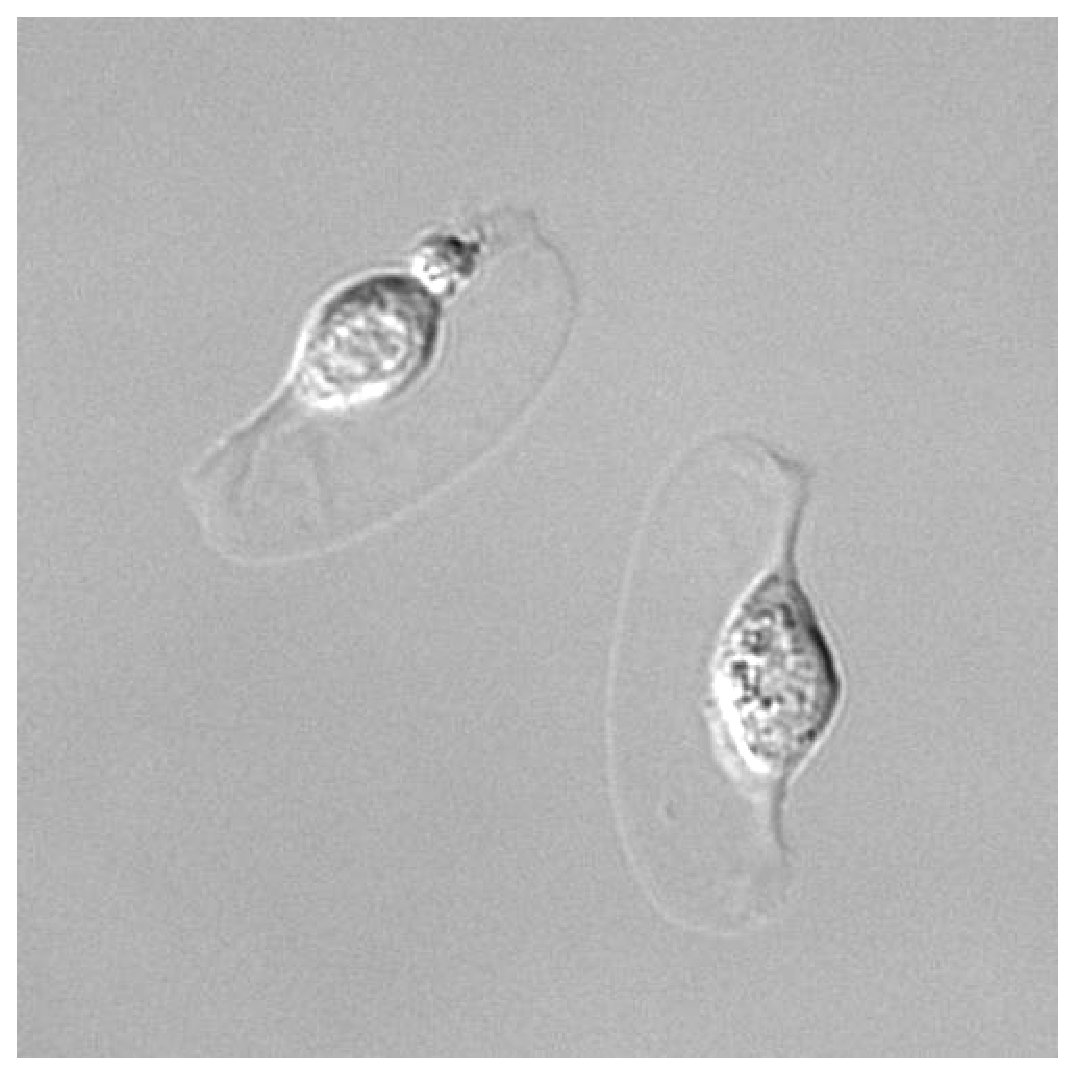
\includegraphics[width=4cm]{kera.eps}
\caption{細胞遊走中のケラトサイト。(撮影:中田多可子氏(岩楯研究室))}
\label{fig:kera}
\end{figure}

\begin{figure}[tbp]
\centering
 \subfloat[]{%
  \begin{tabular}{c}
   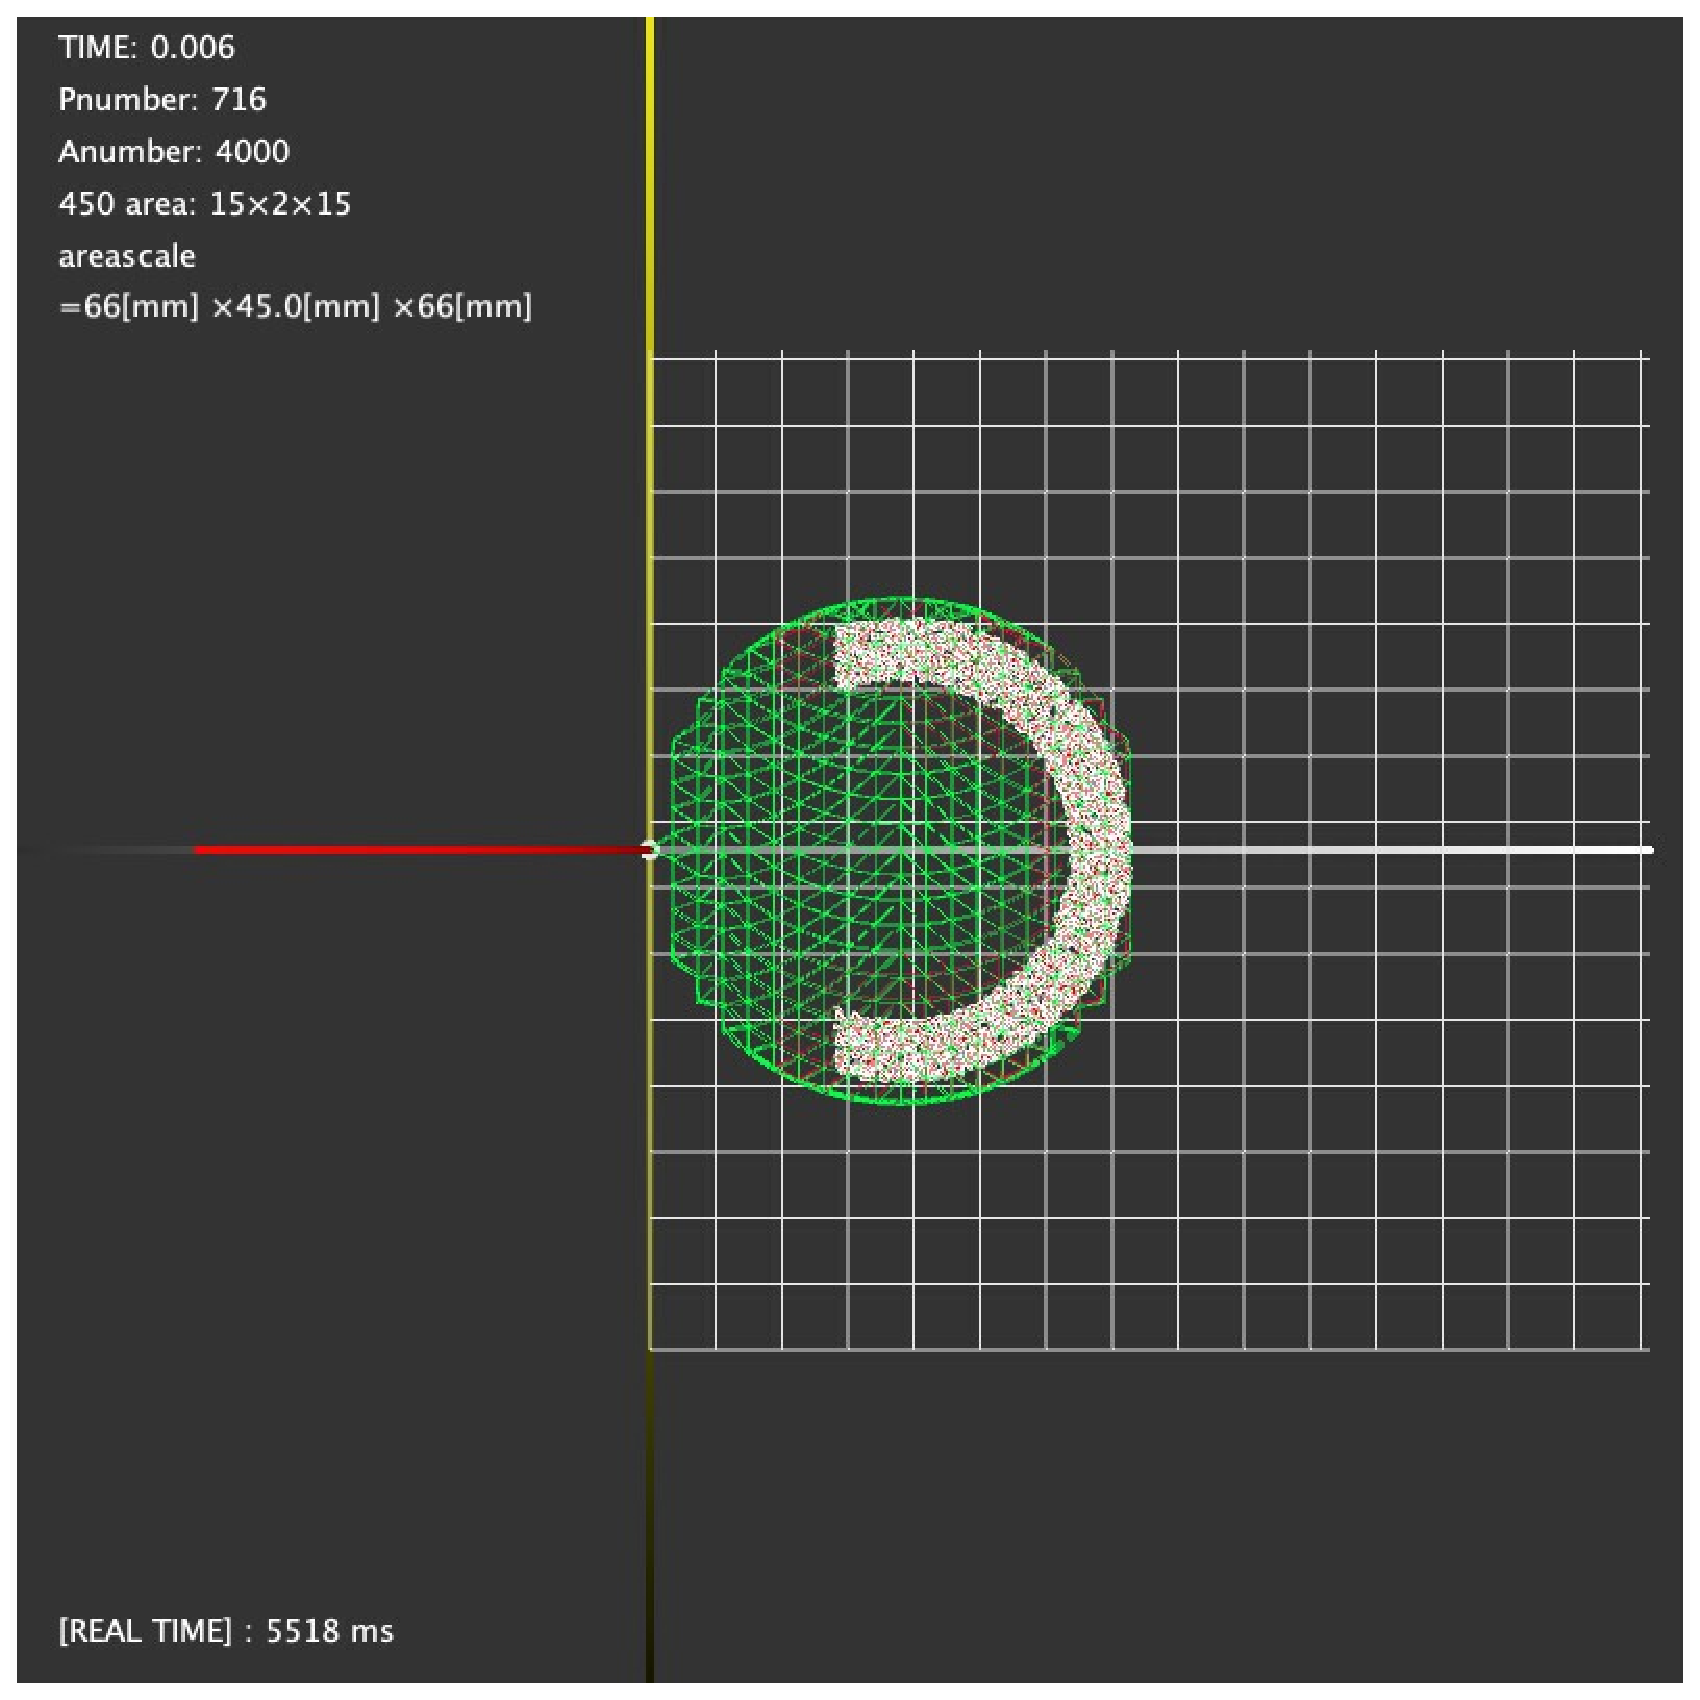
\includegraphics[width=3cm]{top.eps} 
  \end{tabular}
 }%
 \subfloat[]{%
  \begin{tabular}{c}
   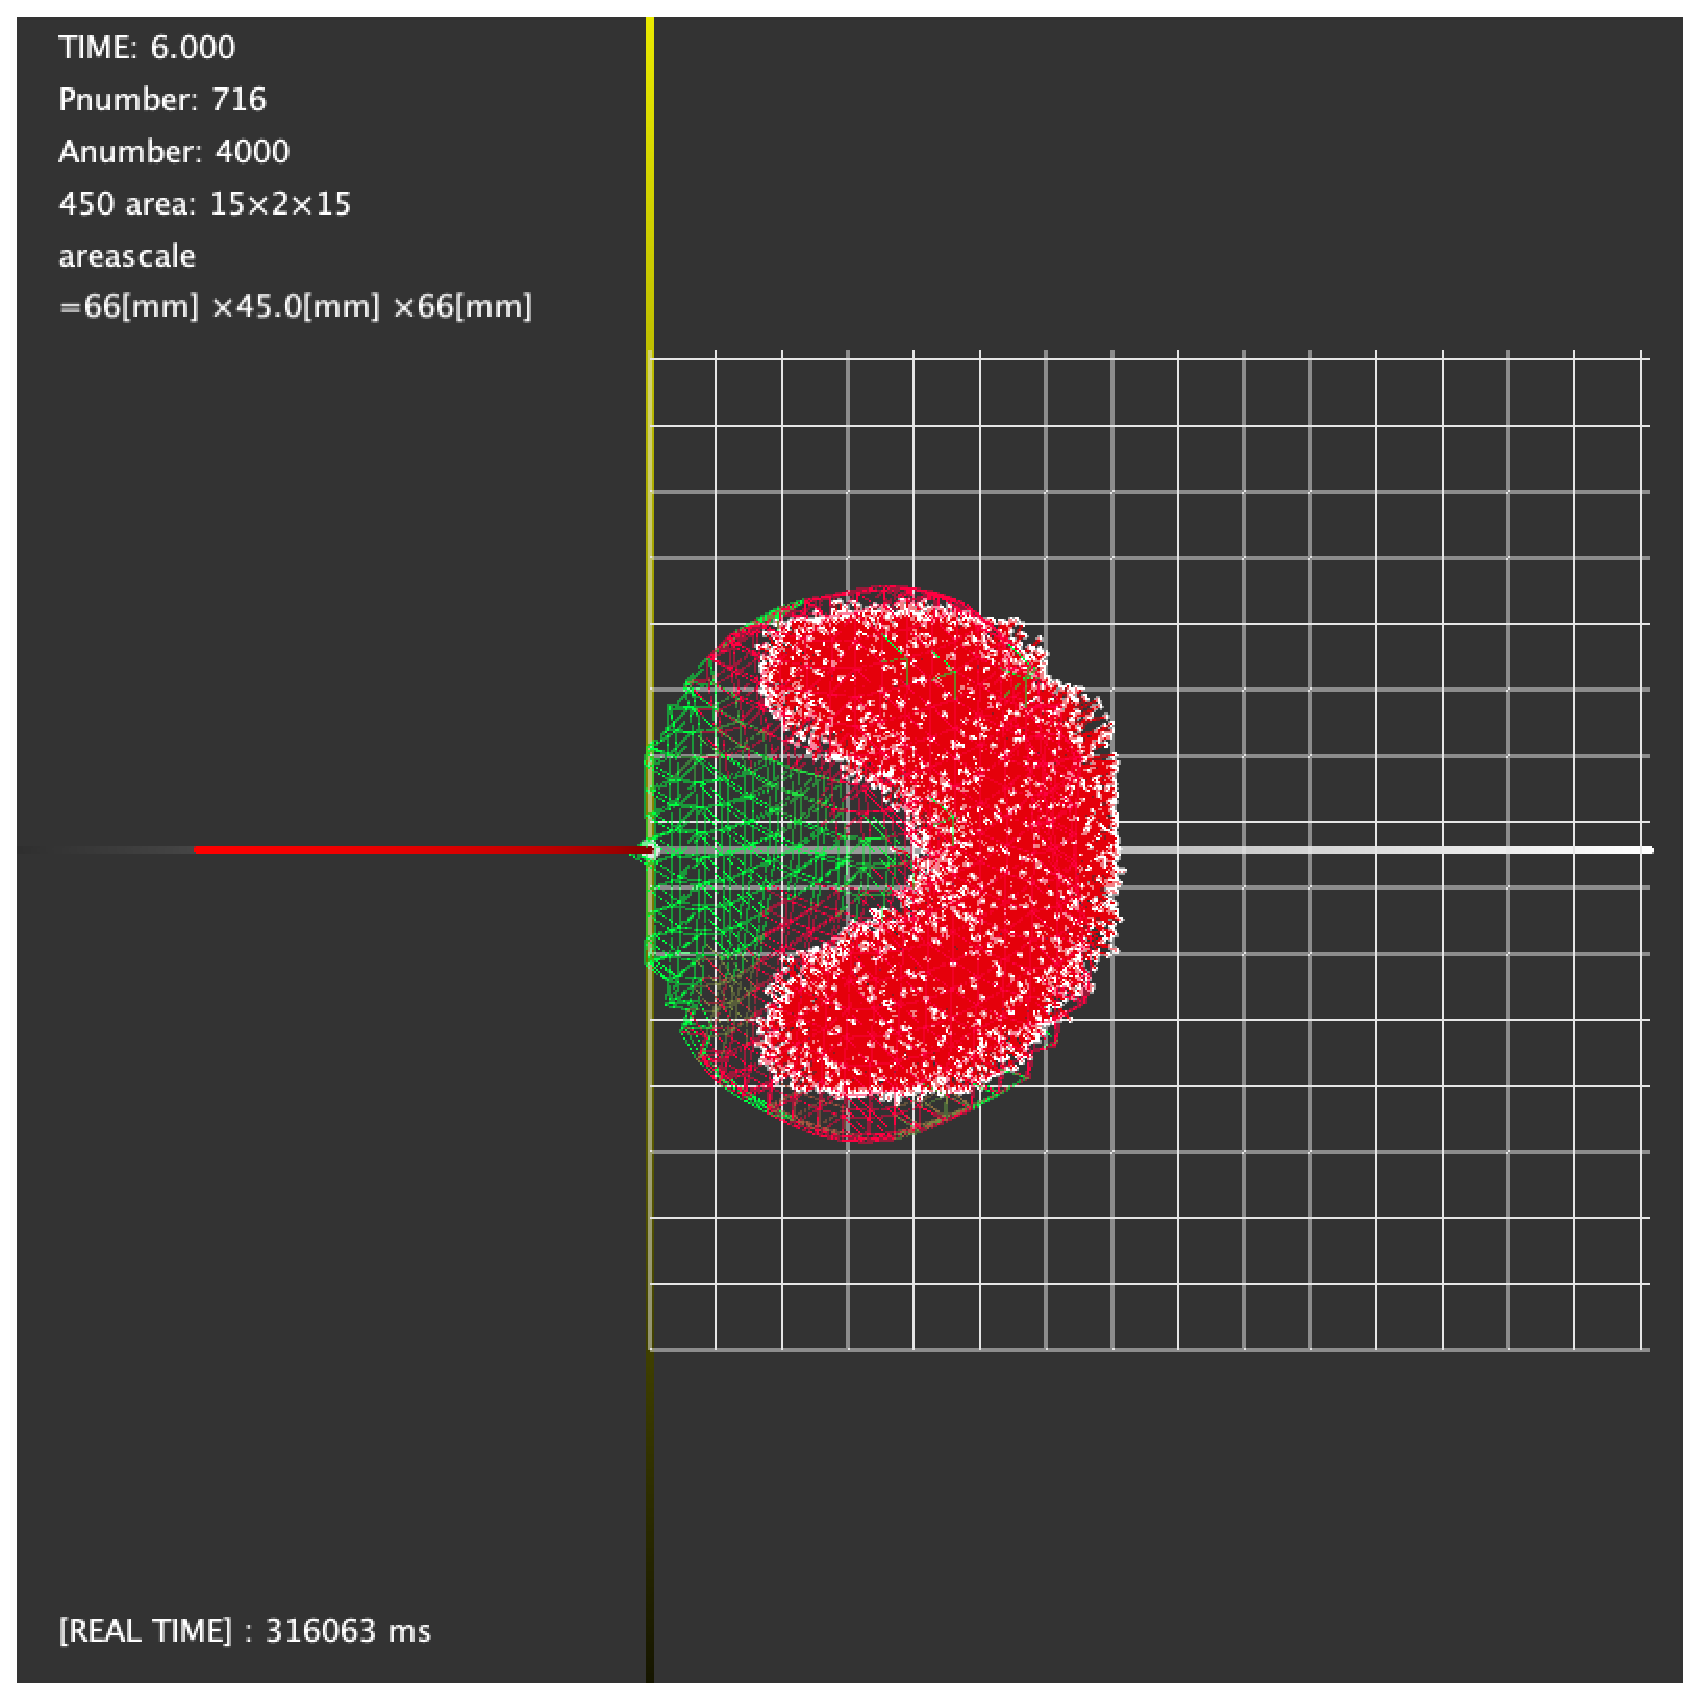
\includegraphics[width=3cm]{top60_arf.eps} 
  \end{tabular}
 }%
 \caption{シミュレーション結果。緑は細胞膜、白は重合前のアクチン分子、赤は重合後のF-actinを示す。(a)~初期配置。膜分子は円柱の表面上、アクチン分子はU字型領域に配置されている。(b)~$t=6.0$~[s]でのシミュレーション結果。アクチン分子が半月状に近い形態に凝集している。}
 \label{fig:res0}
\end{figure}
本研究のシミュレーションでは、細胞膜は互いに相互作用する単純な粒子のネットワークによってモデル化し、初期条件として円柱面上に配置した。細胞膜を構成する各粒子は以下の運動方程式に従って運動すると仮定した。
\begin{equation}
m\frac{d^2\bm{x}_i}{dt^2} = \bm{F}^m_i +  \bm{F}^a_i - \eta \frac{d\bm{x}_i}{dt}
\end{equation}
ここで、$m$は粒子の質量、$\bm{x}_i$の粒子の位置、$\bm{F}^m_i$と$\bm{F}^a_i$はそれぞれ近傍の粒子から受ける弾性力とF-actinから受ける反発力、$\eta$は粘性摩擦係数であり、各変数の添え字$i$は第$i$粒子に対する値であることを示す。

細胞内のアクチン分子は直線上の棒により表現し、重合および脱重合はその一端の確率的伸長゙および他端の収縮によってそれぞれ表現した。初期状態においては、アクチン分子は長さがなく、重合方向はランダムに決定されているとし、細胞後部を除くU字型の領域に一様に配置した。細胞後端より1/5の位置に左右に拡がるSFが存在するとし、アクチン分子からSF両端の二点に向かうベクトルの和の方向に、アクチン分子を確率的に移動させることでARFを表現した。ARFの効果として、アクチン分子の方向をARFの向きに近づける効果も仮定した。

アクチン分子は、アクチン分子密度の低い領域では消滅し細胞膜近くに新たに発生するという条件も設定した。アクチン密度の計算においては、計算量を軽減させるためシミュレーション空間を格子状に分割し(図\ref{fig:res0}の白線)、各領域で密度計算を行った。
\section{結果と考察}
\begin{figure}[tbp]
\centering
 \subfloat[]{%
  \begin{tabular}{c}
   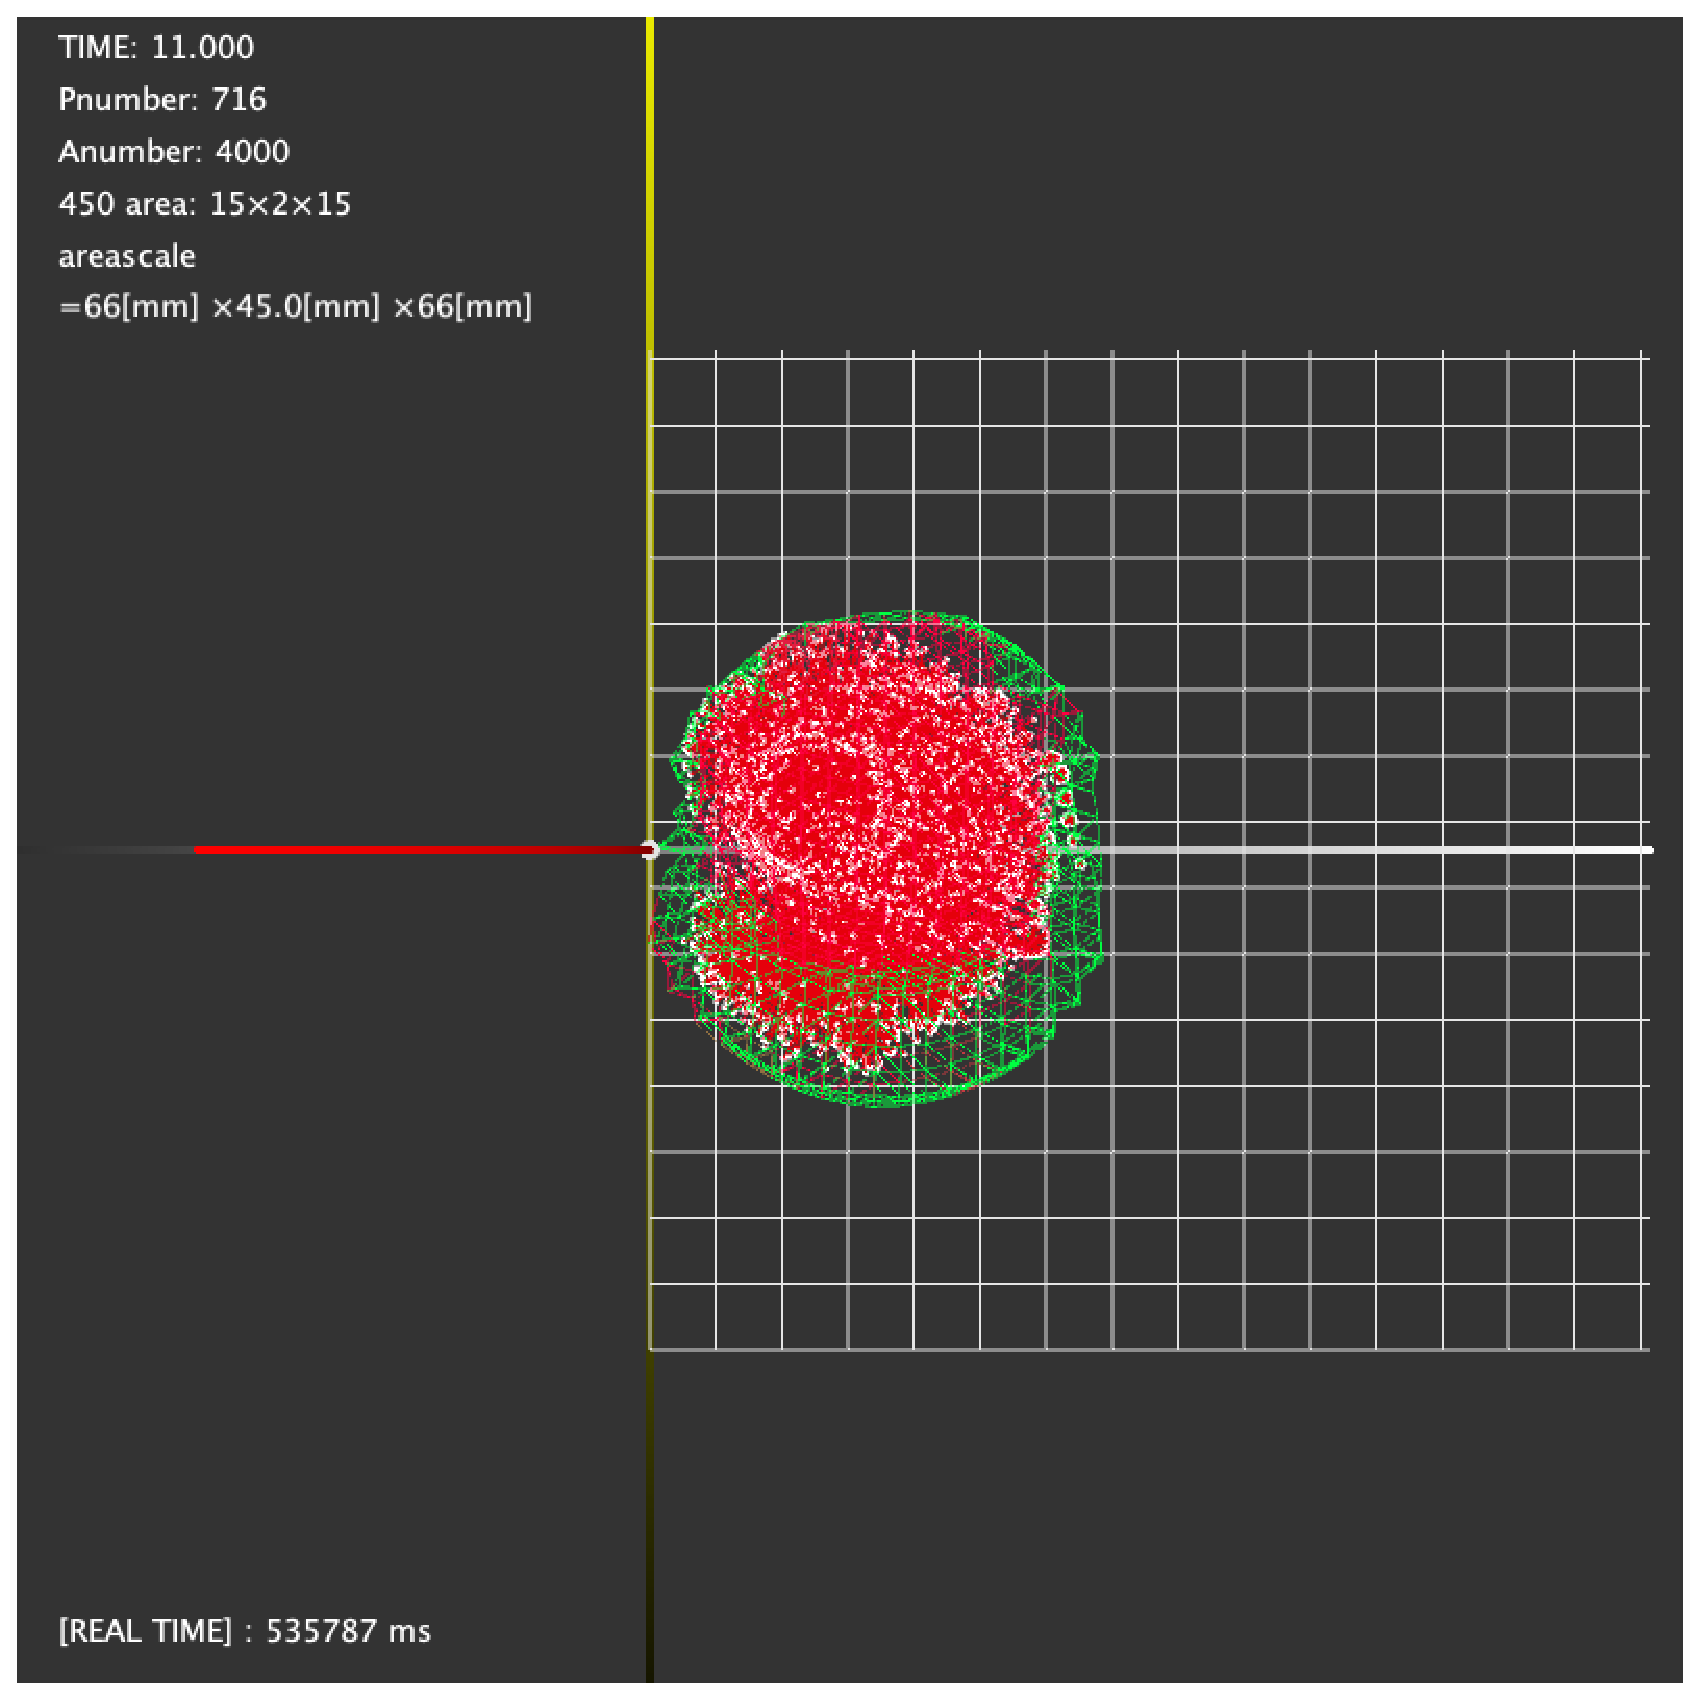
\includegraphics[width=3cm]{1arf.eps} 
  \end{tabular}
 }%
 \subfloat[]{%
  \begin{tabular}{c}
   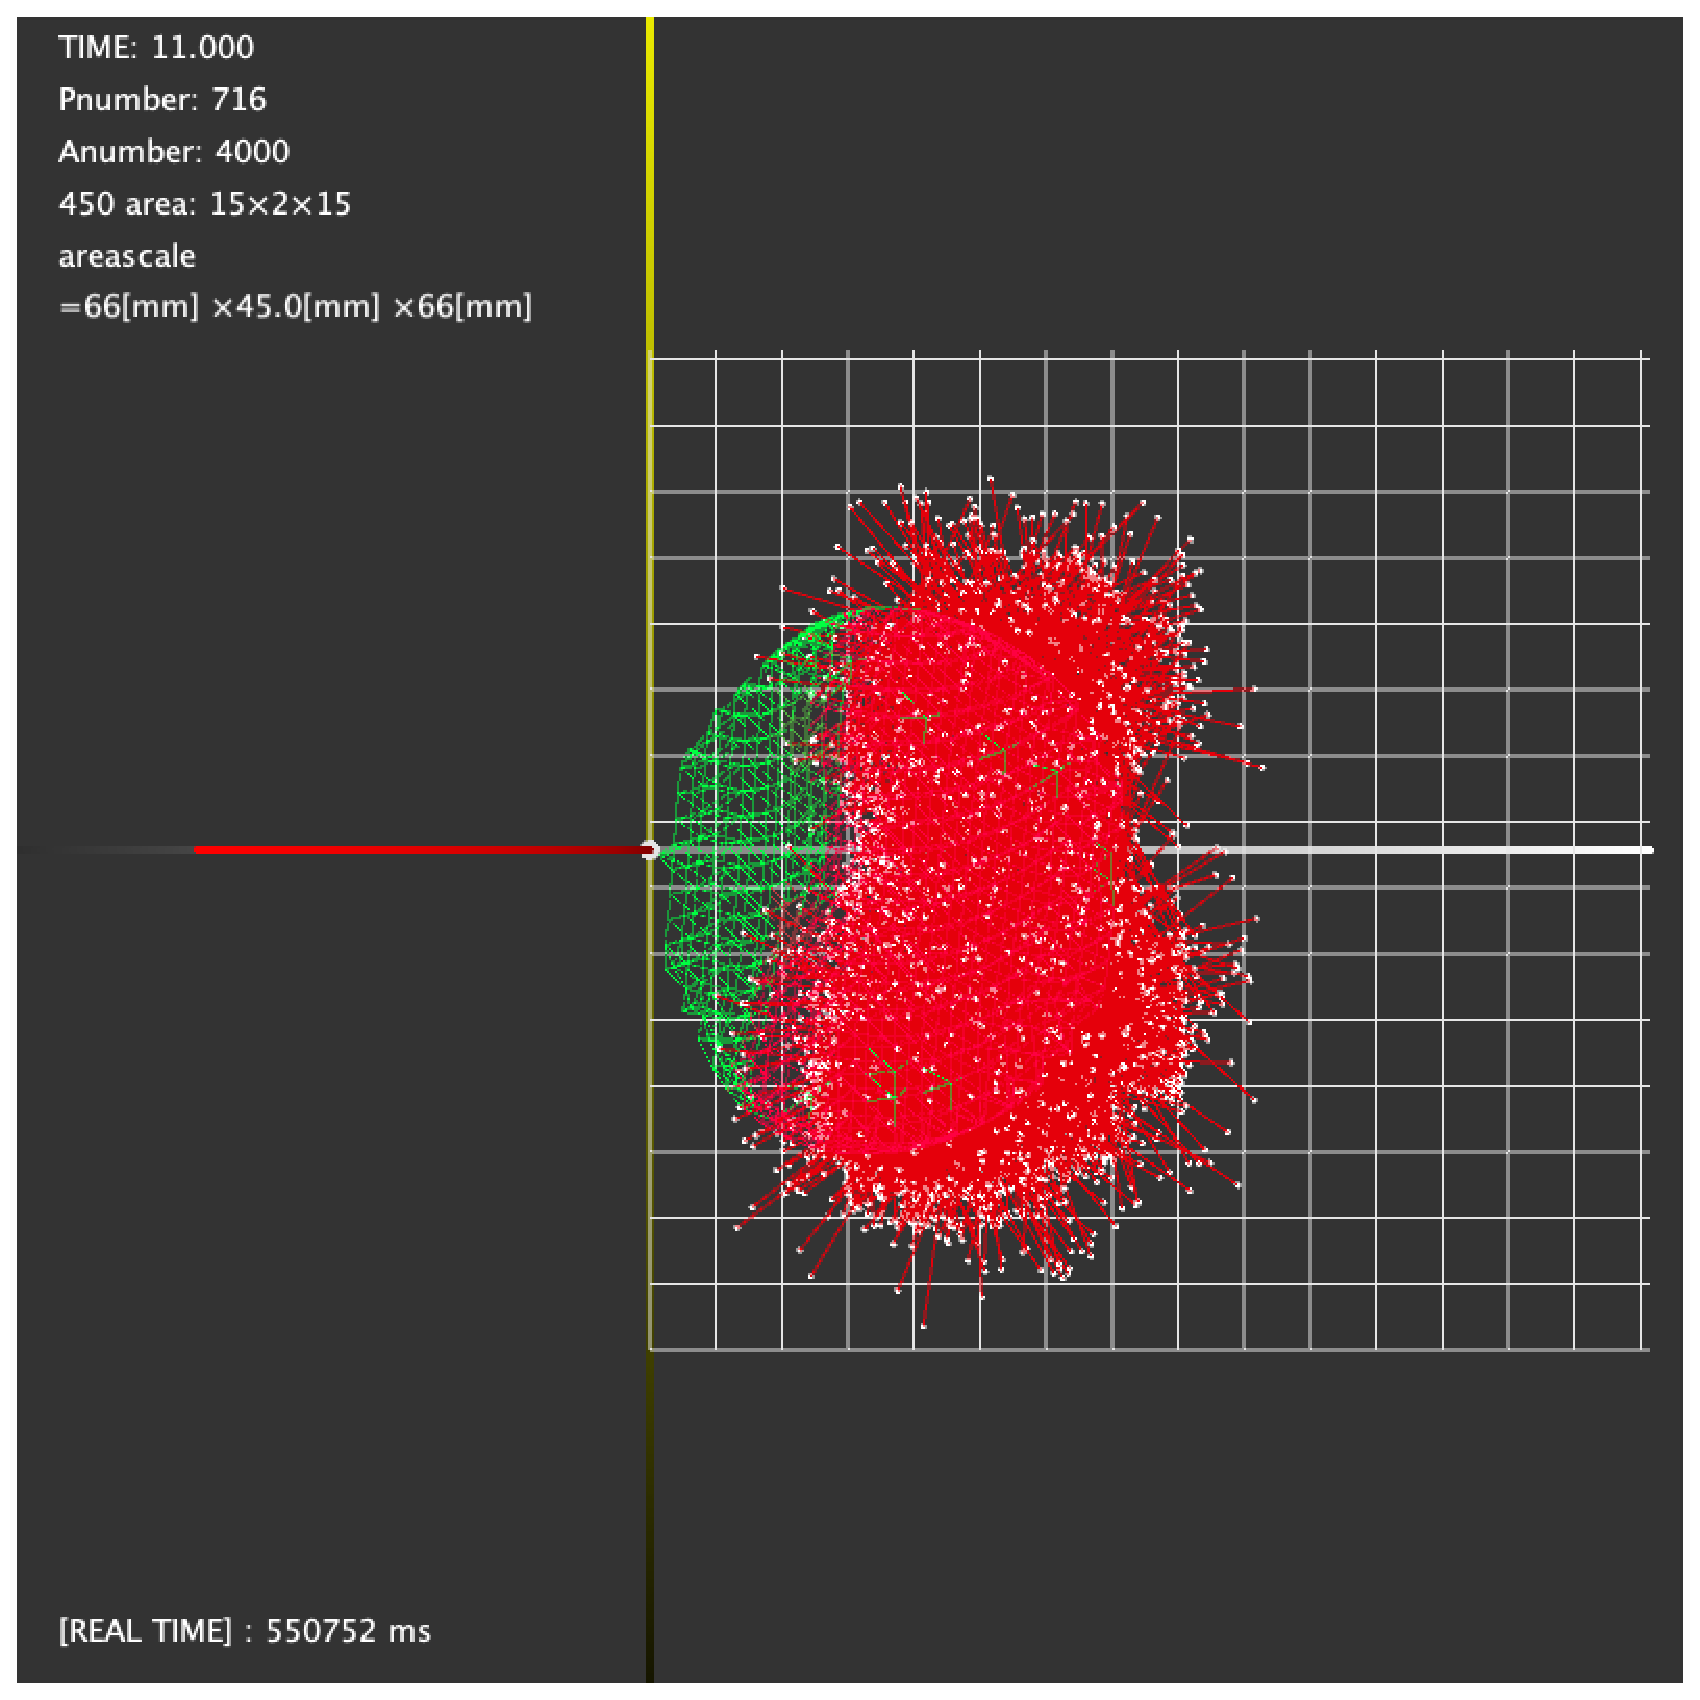
\includegraphics[width=3cm]{narf.eps} 
  \end{tabular}
 }%
  \caption{ARFの諸条件を変更した場合のシミュレーション結果。(a)~SFではなく細胞膜最後部一点に向かって引き戻される場合。(b)~ARF無しの場合。}
 \label{fig:res1}
\end{figure}
シミュレーション実験の結果、アクチン分子は半月状に凝集することが確認できた(図\ref{fig:res0})。図\ref{fig:res1}にARFの設定条件を変更した場合のシミュレーション結果を示す。

ARFの向きをSFから細胞の最後端の点に変更した場合の結果が図~3(a)である。SFの方向に引き戻した場合よりも一点に向かって凝集しようとしている。SFよりもさらに後部の点に向かってアクチン分子が引き戻されるためアクチン分子が細胞全体に広く分布する形となる。半月状の形態とはならないため、細胞遊走の方向も定まらなくなる。ARFを無効化した場合の結果が図~3(b)である。重合方向の修正もアクチン分子の引き戻し効果も無いため、アクチン分子が細胞膜を突き抜けて半月状の形成は出来ない。このようにARFがなければ、アクチン分子は同じ方向へ重合をし続けて細胞膜を突き抜ける。ARFがアクチン分子重合の配向や引き戻し量の調整も行えることから、実際の細胞でそのようなことが起きないのはARFがアクチン重合に対して精密な制御を行っているためであると考えられる。
\bibliographystyle{junsrt}
\begin{thebibliography}{9}
     \bibitem{svitkina1997analysis} T. M. Svitkina, et al.
    ``Analysis of the actin--myosin Ⅱ system in fish epidermal keratocytes: mechanism of cell body translocation''  \sl{J. Cell Biol.} \bf{139}\rm{(2)}, 397-415, 1997.
     \bibitem{yumura1998spatiotemporal} S. Yumura, et al.
    ``Spatiotemporal dynamics of actin concentration during cytokinesis and locomotion in Dictyostelium''  \sl{J. Cell Biol.} \bf{111}\rm{(15)}, 2097-2108, 1998.
  \bibitem{nakashima2015molecular} H. Nakashima, et al.
    ``The molecular dynamics of crawling migration in microtubule-disrupted keratocytes''  \sl{Biophys. and Physicobiol.} \bf{12}\rm{}, 21-29, 2015.
       \bibitem{swaminathan2017actin} V. Swaminathan, et al.
    ``Actin retrograde flow actively aligns and orients ligand-engaged integrins in focal adhesions''  \sl{Proc. Nat. Acad. Sci.} \bf{114}\rm{(40)}, 10648-10653, 2017.
\end{thebibliography}

\end{document}
